\documentclass[12pt]{article}

\usepackage{amsmath,amssymb,amsthm}
\usepackage{geometry}
\usepackage{enumerate}
\usepackage[shortlabels]{enumitem}
\usepackage{graphicx}

\begin{document}
\title{CS 6965 Advanced Data Visualization\\{\bf Project 1}}
\author{Yulong Liang}
\maketitle

\setcounter{section}{1}
\section{The Cat Example (2 pts)}

\begin{enumerate}[label={\bfseries Q\arabic*:}]
\item Some of the small clusters in 20 percent graph will \textbf{disappear} in 80 percent graph, while other clusters will grow \textbf{larger} than before. Moreover, the edges between clusters are \textbf{shorter} in 80 percent graph because the length of edges represent the force between two clusters, i.e., the overlap between two clusters.
\item The total number of clusters increases and the average size of each cluster decreases.
\end{enumerate}

\section{The Bunny Example (3 pts)}

\begin{enumerate}[start=3, label={\bfseries Q\arabic*:}]
\item In the three dimensional point cloud, one of the ear of the bunny is separated from the rest of the body. When clustering, there are \textbf{no overlaps} between that ear and the rest of the body. Thus it results in two connected components.
\item The lens of the data changes from \texttt{sum} to the projection to \texttt{Y-axis}.
\item Yes. For each interval/cube in the space, the algorithm divides the points into two clusters, which leads to 30 clusters instead of 15.
\end{enumerate}

\section{The Digits Example (5 pts)}

\begin{enumerate}[start=6, label={\bfseries Q\arabic*:}]
\item Since \texttt{t-SNE} algorithm initial the data points in the lower dimensional space stochastically, the location of the neighborhoods (a collection of data points which are neighbors) is not identical for each experiment. When using \texttt{DBSCAN} algorithm to cluster the neighborhoods, the ones that are closed to each other will gather into one cluster. Because of the variance of the locations provided by \texttt{t-SNE}, the \texttt{DBSCAN} results are different from time to time.
\item The result using \texttt{Spectral Embedding} produced less and unevenly distributed clusters and within each cluster, the images of different digits are mixed. It did not generate a satifying result.
\item Modifying the parameter to \texttt{n\char`_components=3}. The projected subspace generated by \texttt{Spectral Embedding} was changed from 2-dim to 3-dim, which led to better separated data points. The \texttt{mapper} algorithm will then convert a 3D subspace to a 2D visualization.
\end{enumerate}

\section{Your Own Dataset (5 pts)}
On the Kepler Mapper website, the developer disclosed their future examples: Iris, Diabetes 100k, and Customer purchase behaviour. The first two datasets can be found on UCI Machine Learning Repository, so I picked them to analyze.
\begin{enumerate}
\item \textbf{Iris}
\begin{figure}[h]
\centering
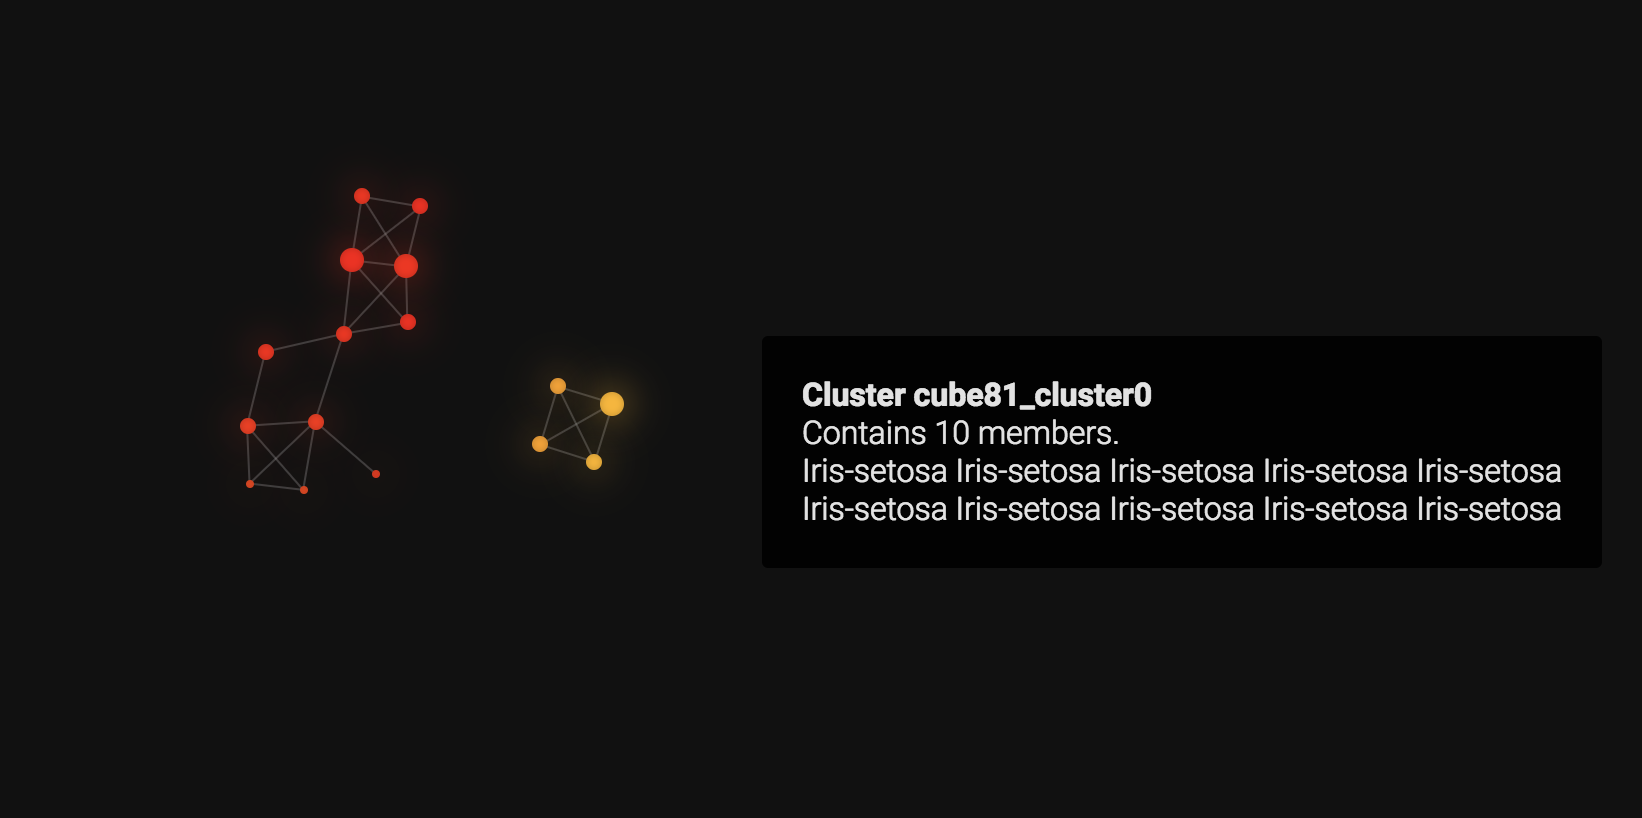
\includegraphics[width=.6\linewidth]{1.png}
\label{fig:name}
\end{figure}\\
\textit{Iris Setosa} can well separated from the other two species in terms of the length and width of petal and sepal. For species of \textit{Iris virginica} and \textit{Iris versicolor}, although a large amount of the flowers are clustered purely, there exists some flowers that are not separable. Those flowers have similar attributes but are different species.

\item \textbf{Diabetes 100k}
\begin{figure}[h]
\centering
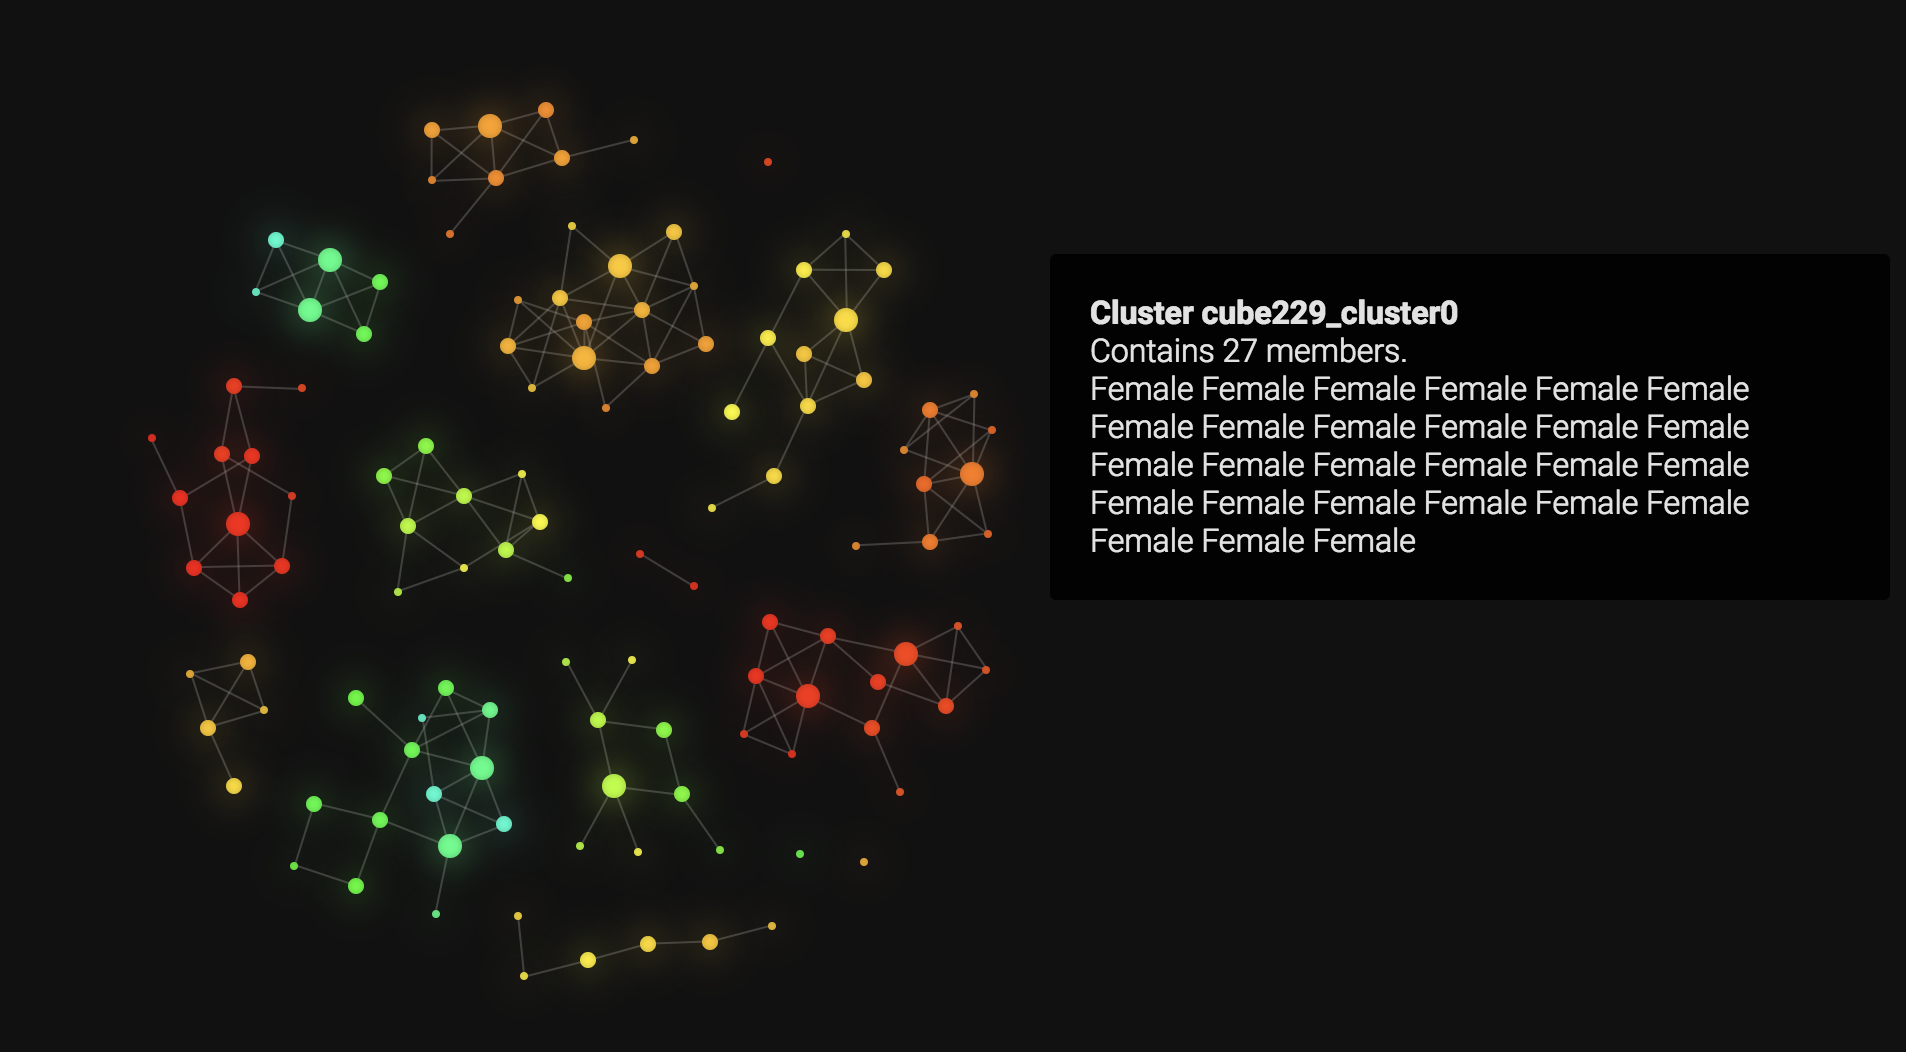
\includegraphics[width=.6\linewidth]{2.png}
\label{fig:name}
\end{figure}\\
Diabete patients are not separable in terms of \textbf{age} and \textbf{race}. However, male patients and female patients never get clustered into the same group, which means diabetes vary quite a lot in terms of \textbf{gender}. 
\end{enumerate}
\end{document}